\chapter{Direkte Lösungsverfahren für dünnbesetzte Gleichungssysteme}
\label{sec:direct_sparse_solvers}

\emph{Problem}: Sei $A \in R^{n \times n}, b \in \R^n$.\\
Finde $x \in \R^n$, sodass $Ax=b$.

Dabei ist $A$ \emph{sehr groß}, dafür aber dünnbesetzt.

\bigskip

\emph{Bisher}: Iterative Verfahren. Funktionieren, im Prinzip, aber
\begin{itemize}
 \item konvergieren nicht für jede invertiere Matrix $A$,
 \item Konvergenzgeschwindigkeit eventuell gering; hängt von der Kondition ab,
 \item Abbruchkriterien nötig, algebraischer Fehler
\end{itemize}

\medskip

\emph{Alternative}: direkte Löser:
\begin{itemize}
 \item Bestimmen die exakte Lösung $x$ nach endlich vielen Schritten (exakte Arithmetik vorausgesetzt)
 \item Beispiel: Gauß-Elimination; funktioniert, nützt aber die Dünnbesetztheit
   von $A$ nicht aus.  Deshalb:
  \begin{itemize}
   \item Hohe Zeitkomplexität ($\mathcal{O} (n^3)$ Schritte)
   \item Großer Speicheraufwand
  \end{itemize}
\end{itemize}

\medskip

\emph{Das Beste beider Welten:} Direkte Löser für dünn besetzte Gleichungssysteme.
\begin{itemize}
 \item Varianten von Gauß- und Cholesky-Elimination
 \item teilweise sehr kompliziert
 \item Zeit- und Speicheraufwand deutlich besser als bei Gauß-Verfahren
 \item Werden in der Praxis sehr häufig verwendet.
 \item Geeignet für Systeme bis ca. $10^5$ Unbekannte, danach zu großer Speicheraufwand
\end{itemize}


\section{Die Multifrontale Methode}

Direktes Lösungsverfahren für dünnbesetzte Matrizen.

\begin{itemize}
 \item Verfahren nach \citet{duff_reid:1983} (1983)
 \item Implementiert z.B. in Matlab, Octave, UMFPack
 \item Wir behandeln nur den Fall das $A$ symmetrisch und positiv definit ist.
 \item Unsere Darstellung folgt \citeauthor{liu:1992}: \citetitle{liu:1992},
       SIAM Review, \citeyear{liu:1992}~\cite{liu:1992}
\end{itemize}

\subsection{Cholesky-Zerlegung}

Die multifrontale Methode basiert auf der Cholesky-Zerlegung.

\medskip

Sei $A$ s.p.d.\ und dünnbesetzt.

\medskip

\emph{Ziel:} Berechne die Cholesky-Zerlegung
\begin{equation*}
 A = LL^T,
 \qquad
 \text{$L$ untere Dreiecksmatrix},
 \qquad
 L_{ii} > 0 \quad \forall i = 1,\dots,n.
\end{equation*}


Wir wiederholen kurz die Cholesky-Zerlegung für vollbesetzte Matrizen.

\medskip

Schreibe dafür $A$ in Blockform
\begin{align*}
 A & =\begin{pmatrix}
        B & V^T \\
        V & C
      \end{pmatrix},
  \qquad B \in \R^{(j-1) \times (j-1)}.
\end{align*}
Dann existiert die Zerlegung
\begin{align*}
 A
 =
 \begin{pmatrix}
  L_B & 0 \\
  VL_B^{-T} & I
 \end{pmatrix}
 \begin{pmatrix}
  I & 0 \\
  0 & C-VB^{-1}V^T
 \end{pmatrix}
 \begin{pmatrix}
  L_B^T & L_B^{-1}V^T \\
  0 & I
 \end{pmatrix}.
\end{align*}
Dabei ist $L_B$ der Cholesky-Faktor von $B$.
\begin{itemize}
 \item Dieser existiert, da $B$ ja s.p.d. ist.
\end{itemize}
\begin{lemma}
\label{lem:rows_of_cholesky_factor}
 Die $n \times (j-1)$-Matrix $\begin{pmatrix}L_B \\ V L_B^{-T}\end{pmatrix}$ besteht
 aus den ersten $j-1$ Spalten von $L$.
\end{lemma}
Die Zerlegung lässt sich rekursiv fortsetzen, denn $C-VB^{-1}V^T$ ist ebenfalls s.p.d.
\begin{proof}[Beweis der Definitheit]
 Sei $u \in \R^{n-j+1}$, $u \neq 0$.  Dann ist
 \begin{equation*}
  u^T(C-VB^{-1}V^T)u
  =
 \begin{pmatrix}
  -B^{-1} V^T u \\ u
 \end{pmatrix}^T
 \begin{pmatrix}
  B & V^T \\ V & C
 \end{pmatrix}
 \begin{pmatrix}
  -B^{-1} V^T u \\ u
 \end{pmatrix}
 >
 0. \qedhere
 \end{equation*}
\end{proof}

Wenn man $j=2$ wählt erhält man
\begin{equation*}
  A
  =
  \begin{pmatrix}
   \sqrt{B} & 0 \\
   \frac{V}{\sqrt{B}} & I
  \end{pmatrix}
  \begin{pmatrix}
   1 & 0 \\
   0 & C-\frac{VV^T}{B}
  \end{pmatrix}
  \begin{pmatrix}
   \sqrt{B} & \frac{V^T}{\sqrt{B}} \\
   0 & I
  \end{pmatrix}
\end{equation*}
\begin{itemize}
 \item Hier ist $B \in \R^{1 \times 1}$ eine Zahl.  Wurzel und Divisions sind also
  wohldefiniert.
 %
 \item Da $\sqrt{B}$ und $V / \sqrt{B}$ billig auszurechnen sind ist also \emph{eine Spalte}
  von $L$ billig auszurechnen.
\end{itemize}

Wegen Lemma~\ref{lem:rows_of_cholesky_factor} gilt
\begin{align*}
  -VB^{-1}V^T
  & =
  -(VL_B^{-T}) (L_B^{-1}V^T) \\
  & =-\sum_{k=1}^{j-1}
 \begin{pmatrix}
  L_{jk} \\
  \vdots \\
  L_{nk}
 \end{pmatrix}
 \begin{pmatrix}
  L_{jk} & \ldots & L_{nk}
 \end{pmatrix}.
\end{align*}

\bigskip

Daraus konstruieren wir einen Algorithmus:
\medskip

\begin{algorithm}[H]
 \SetAlgoLined

 \For{alle Spalten $j=1,\dots,n$}
 {
  Definiere
  \begin{equation*}
  F_j
  \colonequals
  \begin{pmatrix}
   A_{jj} & \dots & A_{jn} \\
   \vdots & & \vdots \\
   A_{nj} & \dots & A_{nn}
  \end{pmatrix}
  -
  \sum_{k=1}^{j-1}
  \begin{pmatrix}
   L_{jk} \\
   \vdots \\
   L_{nk}
  \end{pmatrix}
  \begin{pmatrix}
   L_{jk} & \ldots & L_{nk}
  \end{pmatrix}
  \end{equation*} \\

  Faktorisiere
 \begin{equation*}
  F_j
  =
  \begin{pmatrix}
   L_{jj} & 0 & \dots & 0 \\
   \vdots & & I & \\
   L_{nj} & & &
  \end{pmatrix}
  \begin{pmatrix}
   1 & 0 & \dots & 0 \\
   0 \\
   \vdots & & \widetilde{U}_j \\
   0
  \end{pmatrix}
  \begin{pmatrix}
   L_{jj} & \dots & L_{nj} \\
   0 \\
   \vdots & I & \\
   0 & &
  \end{pmatrix}
 \end{equation*}
 }
\end{algorithm}

\begin{itemize}
 \item In jedem Schritt wird eine weitere Spalte von $L$ bestimmt.
 %
 \item Die Matrix $\widetilde{U}_j$ ergibt sich aus der Faktorisierung.
   Sie wird aber bis auf weiteres nicht weiter verwendet.
\end{itemize}



Wir wollen diesen Algorithmus jetzt so modifizieren, dass er die Dünnbesetztheit von $A$
ausnutzt.

\subsection{Die Struktur von $L$}

Zunächst machen wir uns klar, dass man die Struktur von $L$ bestimmen kann,
ohne $L$ selbst bestimmen zu müssen.

\begin{defi}
 Die Struktur $\mathcal{S}_X$ einer Matrix $X \in \R^{n \times n}$ ist
 \begin{equation*}
  \mathcal{S}_X \colonequals \big\lbrace (i,j) \colon X_{ij} \neq 0 \big\rbrace.
\end{equation*}
\end{defi}
\begin{itemize}
 \item In der tatsächlichen Umsetzung von Matrixalgorithmen im Computer wird man statt der ganzen Matrix $A$ nur deren Struktur $\mathcal{S}_A$ speichern, sowie die dazugehörigen Einträge.
 \item Wie genau, dazu gibt es wieder verschiedene Varianten!
\end{itemize}

Wie sieht die Struktur des Cholesky-Faktors aus?
\begin{satz}
\label{thm:structure_of_cholesky_factor}
Sei $A \in \R^{n \times n}$ s.p.d.\ und $L$ der Cholesky-Faktor.
\begin{enumerate}
 \item Falls $i \leq j$ und $(j,i) \in \mathcal{S}_A$, so ist auch $(j,i) \in \mathcal{S}_L$.
 \item Falls $i<j<k$ und $(j,i) \in \mathcal{S}_L$ und $(k,i) \in \mathcal{S}_L$, dann ist auch $(k,j) \in \mathcal{S}_L$.
\end{enumerate}
Damit sind alle Einträge von $\mathcal{S}_L$ beschrieben.
\end{satz}
\begin{bsp}
\begin{equation*}
	A=\begin{pmatrix}
		\bullet & & & \bullet & & & \bullet \\
		& \bullet & & & & & \bullet \\
		& & \bullet & & \bullet & \bullet & \\
		\bullet & & & \bullet & & & \\
		& & \bullet & & \bullet & & \bullet \\
		& & \bullet & & & \bullet & \\
		\bullet & \bullet & & & \bullet & & \bullet\\
	\end{pmatrix}, \quad L=\begin{pmatrix}
		\bullet & & & & & & \\
		& \bullet & & & & & \\
		& & \bullet & & & & \\
		\bullet & & & \bullet & & & \\
		& & \bullet & & \bullet & & \\
		& & \bullet & & \circ & \bullet & \\
		\bullet & \bullet & & \circ & \bullet & \circ & \bullet
	\end{pmatrix}
\end{equation*}
\end{bsp}
\begin{proof}
Betrachte wieder Darstellung
\begin{equation*}
 A=\begin{pmatrix}
    B & V^T \\
    V & C
\end{pmatrix},
\qquad B \in \R^{1\times 1} = \R.
\end{equation*}
\begin{enumerate}
 \item
  \begin{itemize}
   \item Da $L_{11}=\sqrt{B}$ und $B>0$ enthält $\mathcal{S}_L$ alle Diagonaleinträge.
   \item Da die erste Spalte von $L$ unterhalb der Diagonalen gleich $\frac{V}{\sqrt{B}}$ ist
     enthält $\mathcal{S}_L$ alle Einträge von $\mathcal{S}_A$ unterhalb der Diagonalen.
  \end{itemize}
 \item
   \begin{itemize}
    \item Der Algorithmus berechnet die Cholesky-Zerlegung spaltenweise.
    \item Im $i$-ten Schritt wird die $i$-te Spalte von $L$ berechnet.
       Danach ändert sie sich nicht mehr.
    \begin{equation*}
     \begin{pmatrix}
       & & 0 \\
       \hline
       & L_{ii} & \\
       \hline
       & \tilde{l}_i & \tilde{A}_i - \tilde{l}_i \tilde{l}_i^T
     \end{pmatrix}
    \end{equation*}

    \item Angenommen, $(j,i) \in \mathcal{S}_L$ und $(k,i) \in \mathcal{S}_L$
    \item Dann sind auch $(\tilde{l}_i)_j$ und $(\tilde{l}_i)_k$ Struktureinträge.
    \item Da $(\tilde{l}_i \tilde{l}_i^T)_{jk} = (\tilde{l}_i)_j \cdot (\tilde{l}_i)_k$
     ist dann auch $(\tilde{l}_i \tilde{l}_i^T)_{jk}$ Struktureintrag.
    \item Also ist auch $(\tilde{A}_i-\tilde{l}_i \tilde{l}_i^T)_{jk}$ Struktureintrag.
    \item Mit 1) folgt die Aussage rekursiv. \qedhere
 \end{itemize}
\end{enumerate}
\end{proof}
Was passiert wenn $(\tilde{A}_i - \tilde{l}_i \tilde{l}_i^T)_{jk}$ zufällig gerade
Null ergibt?
\begin{itemize}
 \item Entgegen der Definition von $S_L$ bezeichnet man $(j,k)$ dann dennoch als
  Struktureintrag von $L$.
 \item Vorteil: Man kann dann die Struktur von $L$ nur anhand der Struktur von $A$ bestimmen.
 \item Vermutung: Dieser Fall kommt ohnehin selten vor.
\end{itemize}

\subsection{Ausnutzen der Dünnbesetztheit, Teil~1}

Wir wollen den Algorithmus jetzt so modifizieren, dass er die Dünnbesetztheit von $A$
ausnutzt.

\medskip

\emph{Idee:} Die $j$-te Spalte von $L$ hängt nur von der ersten Zeile und Spalte von $F_j$ ab.

Modifizierter Algorithmus:

\begin{algorithm}[H]
 \SetAlgoLined

 \For{alle Spalten $j=1,\dots,n$}
 {
  Definiere
 \begin{equation*}
  F_j
  \colonequals
  \begin{pmatrix}
   A_{jj} & \dots & \dots & A_{jn} \\
   \vdots & 0 & \dots & 0 \\
   \vdots & \vdots & & \vdots \\
   A_{nj} & 0 & \dots & 0
  \end{pmatrix}
  -
  \sum_{k=1}^{j-1}
  \begin{pmatrix}
   L_{jk} \\
   \vdots \\
   L_{nk}
  \end{pmatrix}
  \begin{pmatrix}
   L_{jk} & \ldots & L_{nk}
  \end{pmatrix}
  \end{equation*}
 \\
 %
 Faktorisiere
 \begin{equation*}
  F_j
  =
  \begin{pmatrix}
   L_{jj} & 0 & \dots & 0 \\
   \vdots & & I & \\
   L_{nj} & & &
  \end{pmatrix}
  \begin{pmatrix}
   1 & 0 & \dots & 0 \\
   0 \\
   \vdots & & \widehat{U}_j \\
   0
  \end{pmatrix}
  \begin{pmatrix}
   L_{jj} & \dots & L_{nj} \\
   0 \\
   \vdots & I & \\
   0 & &
  \end{pmatrix}
 \end{equation*}
 }
\end{algorithm}

Aus $\widetilde{U}_j$ ist eine andere Matrix $\widehat{U}_j$ geworden.
\begin{itemize}
 \item Macht nichts: $\widetilde{U}_j$ wurde ohnehin nicht weiter verwendet.
\end{itemize}

\bigskip

\emph{Idee:} Auch vom zweiten Summanden
\begin{equation*}
  -
  \sum_{k=1}^{j-1}
  \begin{pmatrix}
   L_{jk} \\
   \vdots \\
   L_{nk}
  \end{pmatrix}
  \begin{pmatrix}
   L_{jk} & \ldots & L_{nk}
  \end{pmatrix}
\end{equation*}
ist nur die erste Zeile und Spalte relevant.

Es reicht also, über die Spalten $k=1,\dots,j-1$ zu addieren, für die $L_{jk} \neq 0$ ist.

\medskip

Neuer Algorithmus:

\begin{algorithm}[H]
 \SetAlgoLined

 \For{alle Spalten $j=1,\dots,n$}
 {
 Definiere
 \begin{equation*}
  F_j
  \colonequals
  \begin{pmatrix}
   A_{jj} & \dots & \dots & A_{jn} \\
   \vdots & 0 & \dots & 0 \\
   \vdots & \vdots & & \vdots \\
   A_{nj} & 0 & \dots & 0
  \end{pmatrix}
  -
  \sum_{\substack{k=1 \\ L_{jk} \neq 0}}^{j-1}
  \begin{pmatrix}
   L_{jk} \\
   \vdots \\
   L_{nk}
  \end{pmatrix}
  \begin{pmatrix}
   L_{jk} & \ldots & L_{nk}
  \end{pmatrix}
  \end{equation*}
 \\
 %
 Faktorisiere
 \begin{equation*}
  F_j
  =
  \begin{pmatrix}
   L_{jj} & 0 & \dots & 0 \\
   \vdots & & I & \\
   L_{nj} & & &
  \end{pmatrix}
  \begin{pmatrix}
   1 & 0 & \dots & 0 \\
   0 \\
   \vdots & & \overline{U}_j \\
   0
  \end{pmatrix}
  \begin{pmatrix}
   L_{jj} & \dots & L_{nj} \\
   0 \\
   \vdots & I & \\
   0 & &
  \end{pmatrix}
 \end{equation*}
 }
\end{algorithm}


\subsection{Graphen- und Baumdarstellung}

Die Struktur der Dreiecksmatrix $L$ lässt sich als gerichteter Graph $G=(V,E)$ darstellen mit
$V=\lbrace 1,\ldots,n \rbrace$ und $E=\lbrace (i,j) \colon (j,i) \in \mathcal{S}_L,i>j \rbrace$.

\medskip

Für die Beispielmatrix von oben erhält man: \newline
\begin{center}
\begin{tikzpicture}
\tikzset{vertex/.style = {shape=circle,draw,minimum size=1.5em}}
\tikzset{edge/.style = {->,> = latex'}}
\node[vertex] (a) at  (-2,2) {$1$};
\node[vertex] (b) at  (0,0) {$2$};
\node[vertex] (c) at  (4,2) {$3$};
\node[vertex] (d) at  (-2,0) {$4$};
\node[vertex] (e) at  (2,0) {$5$};
\node[vertex] (f) at  (4,0) {$6$};
\node[vertex] (g) at  (0,-2) {$7$};
\draw[edge] (a) to (d);
\draw[edge] (d) to (g);
\draw[edge] (a) to (g);
\draw[edge] (b) to (g);
\draw[edge] (e) to (g);
\draw[edge] (f) to (g);
\draw[edge] (c) to (e);
\draw[edge] (c) to (f);
\draw[edge] (e) to (f);
\end{tikzpicture}
\end{center}

\bigskip

Wir können also die letzte Version des Algorithmus umschreiben:

\medskip

\begin{algorithm}[H]
 \SetAlgoLined

 \For{alle Spalten $j=1,\dots,n$}
 {
  Definiere
 \begin{equation*}
  F_j
  \colonequals
  \begin{pmatrix}
   \dots
  \end{pmatrix}
  -
  \sum_{\substack{k=1 \\ \text{$\exists$ Kante von $k$ nach $j$}}}^{j-1}
  \begin{pmatrix}
   L_{jk} \\
   \vdots \\
   L_{nk}
  \end{pmatrix}
  \begin{pmatrix}
   L_{jk} & \ldots & L_{nk}
  \end{pmatrix}
  \end{equation*}
 \\
 %
 Faktorisiere [...]
 }
\end{algorithm}

\subsubsection{Der Eliminierungsbaum}

Andererseits ist diese Darstellung teilweise redundant: zwischen zwei Knoten kann es mehr
als einen Weg geben.

Denn: Satz~\ref{thm:structure_of_cholesky_factor} sagt, dass falls es die Kanten
$(i,j)$ und $(i,k)$ gibt mit $j<k$, dann gibt es auch $(j,k)$.

Entferne Kanten solange, bis jeder Knoten nur noch höchstens einen Nachfolger hat.
Und zwar auf eine bestimmte Art:

\begin{defi}
Der Elimiminierungsbaum $T(A)$ von $A$ ist der Baum mit den Knoten $V = \{1,\ldots,n\}$ und Kanten
\begin{equation*}
 E=\big\lbrace (j,p) \colon \mathrm{falls}\ p=\min \lbrace i > j \colon (i,j) \in S_L \rbrace \big\rbrace.
\end{equation*}
\end{defi}

Anschaulich: $p$ ist die Zeile des ersten Eintrags von $L$ in der $j$-ten Spalte (unter der Diagonalen).

Für das Beispiel von eben erhält man:

\begin{center}
\begin{tikzpicture}
\tikzset{vertex/.style = {shape=circle,draw,minimum size=1.5em}}
\tikzset{edge/.style = {->,> = latex'}}
\node[vertex] (a) at  (-2,2) {$1$};
\node[vertex] (b) at  (0,0) {$2$};
\node[vertex] (c) at  (4,2) {$3$};
\node[vertex] (d) at  (-2,0) {$4$};
\node[vertex] (e) at  (2,0) {$5$};
\node[vertex] (f) at  (4,0) {$6$};
\node[vertex] (g) at  (0,-2) {$7$};
\draw[edge] (a) to (d);
\draw[edge] (d) to (g);
\draw[edge] (b) to (g);
\draw[edge] (f) to (g);
\draw[edge] (c) to (e);
\draw[edge] (e) to (f);
\end{tikzpicture}
\end{center}

\begin{satz}
\label{thm:ancestors}
Falls $(j,k) \in \mathcal{S}_L$, dann existiert ein Pfad $k \rightsquigarrow j$ in $T(A)$.
\end{satz}

\begin{defi}
Ein Knoten $i$ heißt Vorgänger von $j$, falls ein Weg $i \rightsquigarrow j$ in $T(A)$ existiert.
Schreibe $T(j)$ für die Menge aller Vorgänger von $j$.
\end{defi}

Mit dieser Terminologie können wir den Algorithmus nochmals umschreiben:

\begin{algorithm}[H]
 \SetAlgoLined

 \For{alle Spalten $j=1,\dots,n$}
 {
  Definiere
 \begin{equation*}
  F_j
  \colonequals
  \begin{pmatrix}
   \dots
  \end{pmatrix}
  -
  \sum_{k \in T(j) \setminus \{j\}}^{j-1}
  \begin{pmatrix}
   L_{jk} \\
   \vdots \\
   L_{nk}
  \end{pmatrix}
  \begin{pmatrix}
   L_{jk} & \ldots & L_{nk}
  \end{pmatrix}
  \end{equation*}
  \\
 %
 Faktorisiere [...]
 }
\end{algorithm}


Die Umkehrung von Satz~\ref{thm:ancestors} gilt nicht unbedingt. So ist im Beispiel
Knoten~3 Vorgänger von Knoten~7, der Eintrag $(3,7)$ existiert aber nicht in $L$.
Der Wechsel zum Eliminierungsbaum führt also erstmal wieder überflüssige Rechenoperationen
ein.  Im endgültigen Algorithmus sind die aber wieder verschwunden (s.u.).

\subsection{Ausnutzen der Dünnbesetztheit, Teil~2}

\emph{Idee:} Jeder Summand in $F_j$ ist für sich dünnbesetzt.

\medskip

\emph{Aber:} Jeder Summand hat doch vermutlich eine andere Besetzungsstruktur?
 Die \emph{Summe} ist doch vermutlich dann doch relativ dicht?

\medskip

\emph{Nein!}

\begin{satz}
\label{thm:column_structure_inclusion}
Seien $i$ und $j$ Knoten in $T(A)$, sodass ein Pfad $i \rightsquigarrow j$ existiert (also $i<j$).
Dann sind alle Struktureinträge der $i$-ten Spalte von $L$ (unterhalb der $j$-ten Zeile) in der
Struktur der $j$-ten Spalte enthalten
\begin{equation*}
 (k,i) \in \mathcal{S}_L
 \implies
 (k,j) \in \mathcal{S}_L \qquad (\text{falls $k \geq j$ und $i \rightsquigarrow j$}).
\end{equation*}
\end{satz}

\bigskip

Seien also
\begin{equation*}
 j = i_0 < i_1 < \dots < i_r
\end{equation*}
die Zeilen der Einträge der $j$-ten Spalte von $L$.

Neuer Algorithmus:

\medskip

\begin{algorithm}[H]
 \SetAlgoLined

 \For{alle Spalten $j=1,\dots,n$}
 {
  Definiere
 \begin{equation*}
  F_j
  \colonequals
  \begin{pmatrix}
   A_{i_0 i_0} & \dots & \dots & A_{i_0 i_r} \\
   \vdots & 0 & \dots & 0 \\
   \vdots & \vdots & & \vdots \\
   A_{i_r i_0} & 0 & \dots & 0
  \end{pmatrix}
  -
  \sum_{k \in T(j) \setminus \{ j \}}^{j-1}
  \begin{pmatrix}
   L_{i_0k} \\
   \vdots \\
   L_{i_r k}
  \end{pmatrix}
  \begin{pmatrix}
   L_{i_0 k} & \ldots & L_{i_r k}
  \end{pmatrix}
  \end{equation*}
 \\
 %
 Faktorisiere
 \begin{equation*}
  F_j
  =
  \begin{pmatrix}
   L_{i_0 j} & 0 & \dots & 0 \\
   \vdots & & I & \\
   L_{i_r j} & & &
  \end{pmatrix}
  \begin{pmatrix}
   1 & 0 & \dots & 0 \\
   0 \\
   \vdots & & U_j \\
   0
  \end{pmatrix}
  \begin{pmatrix}
   L_{i_0 j} & \dots & L_{i_rj} \\
   0 \\
   \vdots & I & \\
   0 & &
  \end{pmatrix}
 \end{equation*}
 }
\end{algorithm}

Die Matrizen $F_j \in \R^{(r+1) \times (r+1)}$ und $U_j \in \R^{r \times r}$ sind
jetzt vollbesetzt.
\begin{itemize}
 \item $F_j$ nennt man $j$-te \emph{Frontal-Matrix}
 \item $U_j$ nennt man $j$-te \emph{Update-Matrix}.
\end{itemize}


\subsection{Matrix-Superposition (Der extend-add Operator)}
Wir brauchen noch ein Werkzeug zum Arbeiten mit den neuen Matrizen.

\begin{itemize}
 \item Die aktuelle Definition von $F_j$ sagt, dass man den kompletten Teilbaum von $T(A)$ in $j$ abläuft und für jeden Knoten Matrizen aufstellt.
 \item Das kann immer noch ziemlich teuer sein.
 \item Hier kommt der Trick: Man kann $F_j$ effizient aus den Update-Matrizen der \emph{direkten} Vorgänger
   zusammenbauen!
\end{itemize}

\begin{itemize}
 \item Sei $R \in \R^{r \times r}$ mit $r \leq n,S \in \R^{s \times s}$ mit $s \leq n$.
 \item Jede Zeile/Spalte von $R$ und $S$ soll zu einer Zeile/Spalte der gegebenen Matrix $A$ gehören
 \item Indexmengen: $i_1<\ldots<i_r$ für $R$, \\ $j_1<\ldots<j_s$ für $S$
 \item[1)] Sei $k_1<\ldots < k_t$ die Vereinigung der beiden Indexmengen
 \item[2)] Passe $R$ und $S$ an die Indexmenge $k_1<\ldots<k_t$ an, indem Nullzeilen und Nullspalten eingefügt werden.
 \item[3)] Definiere $R \extendadd S \in \R^{t \times t}$ als Summe der erweiterten Matrizen $R,S$.
\end{itemize}

Der Operator $\extendadd$ wird in der englischsprachigen Literatur als \glqq extend--add\grqq{}
bezeichnet.

\begin{bsp}
\begin{equation*}
 R
 =
 \begin{pmatrix}
  p & q \\
  u & v
 \end{pmatrix},
 \qquad
 S
 =
 \begin{pmatrix}
  w & x \\
  y & z
 \end{pmatrix}
\end{equation*}
Indexmengen $\{5,8\}$ bzw.\ $\{5,0\}$.

Dann hat $R \extendadd S$ die Indexmenge $\lbrace 5,8,9 \rbrace$, und
\begin{equation*}
 R \extendadd S
 =
 \begin{pmatrix}
  p & q & 0 \\
  u & v & 0 \\
  0 & 0 & 0
 \end{pmatrix}
 +
 \begin{pmatrix}
  w & 0 & x \\
  0 & 0 & 0 \\
  y & 0 & z
 \end{pmatrix}
 =
 \begin{pmatrix}
  p+w & q & x \\
  u & v & 0 \\
  y & 0 & z
 \end{pmatrix}
\end{equation*}
\end{bsp}
Damit kann man eine billigere Formel für $F_j$ finden.
\begin{satz}[{\citet[Thm.\,4.1]{liu:1992}}]
\label{thm:frontal_matrix_children}
Seien $c_1, \ldots,c_s$ die \emph{direkten} Vorgänger des Knotens $j$ im Eliminierungsbaum $T(A)$ von $A$. Dann ist
\begin{equation*}
 F_j
 =
 \begin{pmatrix}
  A_{{i_0}{i_0}} & A_{{i_0}{i_1}} & \ldots & A_{{i_0}{i_r}} \\
  A_{{i_1}{i_0}} \\
  \vdots & & 0 \\
  A_{{i_r}{i_0}}
 \end{pmatrix} \extendadd U_{c_1} \extendadd U_{c_2} \extendadd \ldots \extendadd U_{c_s}.
\end{equation*}
\end{satz}

Zum Beweis braucht man:

\begin{satz}[{\citeauthor[Thm.\,3.3]{liu:1992}}]
Es gilt \begin{equation*}
	U_j=-\sum_{k \in T(j)} \begin{pmatrix}
		L_{i_1k} \\
		\vdots \\
		L_{i_rk}
	\end{pmatrix}
	\begin{pmatrix}
		L_{i_1k} & \ldots & L_{i_rk}
	\end{pmatrix}.
\end{equation*}
\end{satz}
\begin{proof}
Umformen der Zerlegung von $F_j$ gibt
\begin{equation*}
 F_j=\begin{pmatrix}
		L_{i_0j} \\
		\vdots \\
		L_{i_rj}
	\end{pmatrix} \begin{pmatrix}
		L_{i_0j} & \ldots & L_{i_rj}
	\end{pmatrix}+\begin{pmatrix}
		0 & 0 \\
		0 & U_j
	\end{pmatrix}
\end{equation*}
Aber $F_j$ und $U_j$ unterscheiden sich nur in der ersten Zeile und Spalte.

Deshalb
\begin{align*}
 [ & \text{$F_j$ ohne erste Zeile und Spalte}]  \\
 & =
 [ \text{$\overline{U}_j$ ohne erste Zeile und Spalte}] \\
 & =
 \bigg[ \text{$\displaystyle  -\sum_{k \in T(j) \setminus \lbrace j \rbrace}
 \begin{pmatrix}
		L_{i_0 k} \\
		\vdots \\
		L_{i_r k}
	\end{pmatrix} \begin{pmatrix}
		L_{i_0 k} & \dots & L_{i_r k}
 \end{pmatrix}$ ohne erste Zeile und Spalte}\bigg] \\
 %
 & =
 -\sum_{k \in T(j)} \begin{pmatrix}
		L_{i_1k} \\
		\vdots \\
		L_{i_rk}
	\end{pmatrix} \begin{pmatrix}
		L_{i_1k} & \ldots & L_{i_rk}
	\end{pmatrix}=\begin{pmatrix}
		L_{i_1j} \\
		\vdots \\
		L_{i_rj}
	\end{pmatrix} \begin{pmatrix}
		L_{i_1j} & \ldots & L_{i_rj}
	\end{pmatrix}+U_j.
\end{align*}
Daraus folgt die Behauptung.
\end{proof}

\todoannot{1.2\baselineskip}{Es fehlt noch der (kurze) Beweis von Satz~\ref{thm:frontal_matrix_children}.}

\subsection{Der endgültige Algorithmus}

Berechne zunächst die Struktur von $L$.

\medskip

Danach:

\medskip

\begin{algorithm}[H]
 \SetAlgoLined

 \For{alle Spalten $j=1,\dots,n$}
 {
 Seien $i_0,\ldots,i_r$ die Zeilenindizes der Einträge von $L_{*j}$. Nicht vergessen: $i_0=j$
 \\
 %
 Seien $c_1,\ldots,c_s$ die direkten Vorgänger von $j$ im Eliminationsbaum $T(A)$ von $A$.
 \\
 %
 Bilde Frontal-Matrix $F_j$ wie in Satz~\ref{thm:frontal_matrix_children}
  \begin{equation*}
 F_j
 =
 \begin{pmatrix}
  A_{{i_0}{i_0}} & A_{{i_0}{i_1}} & \ldots & A_{{i_0}{i_r}} \\
  A_{{i_1}{i_0}} \\
  \vdots & & 0 \\
  A_{{i_r}{i_0}}
 \end{pmatrix} \extendadd U_{c_1} \extendadd U_{c_2} \extendadd \ldots \extendadd U_{c_s}.
\end{equation*}
 \\
 %
 Faktorisiere
 \begin{equation*}
 F_j
 =
			\begin{pmatrix}
				L_{{i_0}{i_0}} & 0 & \ldots & 0 \\
				L_{{i_1}{i_0}} \\
				\vdots & & I \\
				L_{{i_r}{i_0}}
			\end{pmatrix}
 \begin{pmatrix}
				1 & 0 & \ldots & 0 \\
				0 \\
				\vdots & & U_j \\
				0
 \end{pmatrix}
 \begin{pmatrix}
				L_{{i_0}{i_0}} & L_{{i_1}{i_0}} & \ldots & L_{{i_r}{i_0}} \\
				0 \\
				\vdots & & I \\
				0
 \end{pmatrix}
 \end{equation*}
 \\
 %
 Man merke sich $U_j$, falls nötig.
 }
\end{algorithm}
Das Ergebnis im $j$-ten Schritt ist also: $L_{i_0i_0},\ldots,L_{i_ri_0}$ und $U_j$.

\subsection{Umsortierungen der Matrix}
\begin{itemize}
	\item Die Matrixspalten werden von $1$ bis $n$ behandelt
	\item Die Update-Matrizen werden in eben dieser Reihenfolge erzeugt
	\item Wird eine Matrix $U_j$ nicht für $F_{j+1}$ gebraucht, so muss sie zwischengespeichert werden.
	\item Das verbraucht Speicher!
\end{itemize}
Sei beispielsweise \begin{equation*}
	A=\begin{pmatrix}
		a & & & & & & \bullet & \bullet & \bullet \\
		& b & & \bullet & & \bullet & & & \\
		& & c & & \bullet & & & \bullet & \\
		& \bullet & & d & & & & \bullet & \bullet \\
		& & \bullet & & e & \bullet & & \bullet & \\
		& \bullet & & & \bullet & f & & & \bullet \\
		\bullet & & & & & & g & \bullet & \bullet \\
		\bullet & & \bullet & \bullet & \bullet & & \bullet & h & \\
		\bullet & & & \bullet & & \bullet & \bullet & & i \\
	\end{pmatrix},
 \qquad
 L=\begin{pmatrix}
		a & & & & & & & & \\
		& b & & & & & & & \\
		& & c & & & & & & \\
		& \bullet & & d & & & & & \\
		& & \bullet & & e & & & & \\
		& \bullet & & \circ & \bullet & f & & & \\
		\bullet & & & & & & g & & \\
		\bullet & & \bullet & \bullet & \bullet & \circ & \bullet & h & \\
		\bullet & & & \bullet & & \bullet & \bullet & \circ & i \\
	\end{pmatrix}
\end{equation*}
Eliminierungsbaum:
\newline
\begin{tikzpicture}

\tikzset{vertex/.style = {shape=circle,draw,minimum size=1.5em}}
\tikzset{edge/.style = {->,> = latex'}}

% vertices
\node[vertex] (v1) at  (-2,6) {$1$};
\node[vertex] (v2) at  (2,6) {$2$};
\node[vertex] (v3) at  (6,6) {$3$};
\node[vertex] (v4) at  (2,4) {$4$};
\node[vertex] (v5) at  (6,4) {$5$};
\node[vertex] (v6) at  (4,2) {$6$};
\node[vertex] (v7) at  (-2,4) {$7$};
\node[vertex] (v8) at  (0,0) {$8$};
\node[vertex] (v9) at  (0,-2) {$9$};

%edges
\draw[edge] (v1) to (v7);
\draw[edge] (v2) to (v4);
\draw[edge] (v3) to (v5);
\draw[edge] (v4) to (v6);
\draw[edge] (v5) to (v6);
\draw[edge] (v6) to (v8);
\draw[edge] (v7) to (v8);
\draw[edge] (v8) to (v9);
\end{tikzpicture}
\newline
Z.B.: $F_4$ benutzt nur $U_2$, d.h. $U_1$ und $U_3$ müssen temporär zwischengespeichert werden. \\
\emph{Idee}: Sortiere die Zeilen und Spalten von $A$ so um, dass zu jedem Zeitpunkt möglichst wenig Matrizen $U_j$ gespeichert werden müssen. \begin{equation*}
	\overline{A}=\begin{pmatrix}
		a & \bullet & & & & & & \bullet & \bullet \\
		\bullet & g & & & & & & \bullet & \bullet \\
		& & b & \bullet & & & \bullet & & \\
		& & \bullet & d & & & & \bullet & \bullet \\
		& & & & c & \bullet & & \bullet & \\
		& & & & \bullet & e & \bullet & \bullet & \\
		& & \bullet & & & \bullet & f & & \bullet \\
		\bullet & \bullet & & \bullet & \bullet & \bullet & & h & \\
		\bullet & \bullet & & \bullet & & & \bullet & & i \\
	\end{pmatrix},
 \qquad
 \overline{L}=\begin{pmatrix}
		a & & & & & & & & \\
		\bullet & g & & & & & & & \\
		& & b & & & & & & \\
		& & \bullet & d & & & & & \\
		& & & & c & & & & \\
		& & & & \bullet & e & & & \\
		& & \bullet & \circ & & \bullet & f & & \\
		\bullet & \bullet & & \bullet & \bullet & \bullet & \circ & h & \\
		\bullet & \bullet & & \bullet & & & \bullet & \circ & i \\
	\end{pmatrix}
\end{equation*}
Eliminierungsbaum:
\newline
\begin{tikzpicture}

\tikzset{vertex/.style = {shape=circle,draw,minimum size=1.5em}}
\tikzset{edge/.style = {->,> = latex'}}

% vertices
\node[vertex] (v1) at  (-2,6) {$1$,a};
\node[vertex] (v3) at  (2,6) {$3$,b};
\node[vertex] (v5) at  (6,6) {$5$,c};
\node[vertex] (v4) at  (2,4) {$4$,d};
\node[vertex] (v6) at  (6,4) {$6$,e};
\node[vertex] (v7) at  (4,2) {$7$,f};
\node[vertex] (v2) at  (-2,4) {$2$,g};
\node[vertex] (v8) at  (0,0) {$8$,h};
\node[vertex] (v9) at  (0,-2) {$9$,i};

%edges
\draw[edge] (v1) to (v2);
\draw[edge] (v2) to (v8);
\draw[edge] (v3) to (v4);
\draw[edge] (v4) to (v7);
\draw[edge] (v5) to (v6);
\draw[edge] (v6) to (v7);
\draw[edge] (v7) to (v8);
\draw[edge] (v8) to (v9);
\end{tikzpicture}
\newline
Mit dieser Nummerierung können die Matrizen $U_j$ in einem Stapel (engl.: Stack), einer bestimmten Datenstruktur gespeichert werden. \newline
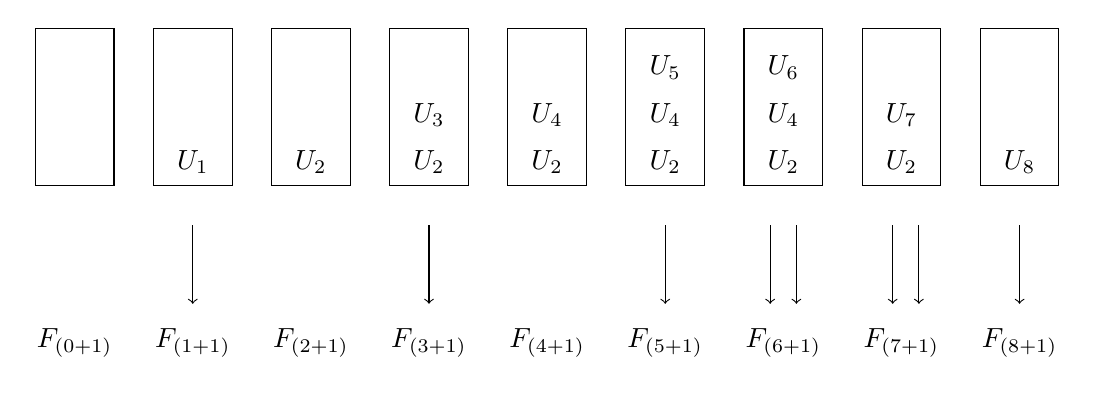
\begin{tikzpicture}
% stacks
\foreach \r in {0,1,...,8}
	\draw (1.5*\r,0) -- (1+1.5*\r,0) -- (1+1.5*\r,2) -- (1.5*\r,2) -- cycle;
% frontal matrices
\foreach \r in {0,1,...,8}
	\draw (1.5*\r+.5,-2)
		node []
			{$F_{(\r+1)}$};
% single arrows
\draw[->] (2,-0.5) -- (2,-1.5);
\draw[->] (5,-0.5) -- (5,-1.5);
\draw[->] (8,-0.5) -- (8,-1.5);
\draw[->] (12.5,-0.5) -- (12.5,-1.5);
% double arrows
\draw[->] (10.889,-0.5) -- (10.889,-1.5);
\draw[->] (11.222,-0.5) -- (11.222,-1.5);
\draw[->] (9.333,-0.5) -- (9.333,-1.5);
\draw[->] (9.666,-0.5) -- (9.666,-1.5);
% nodes in stacks
\draw (2,0.3)
	node []
		{$U_1$};
\draw (3.5,0.3)
	node []
		{$U_2$};
\draw (5,0.3)
	node []
		{$U_2$};
\draw (5,0.9)
	node []
		{$U_3$};
\draw (6.5,0.3)
	node []
		{$U_2$};
\draw (6.5,0.9)
	node []
		{$U_4$};
\draw (8,0.3)
	node []
		{$U_2$};
\draw (8,0.9)
	node []
		{$U_4$};
\draw (8,1.5)
	node []
		{$U_5$};
\draw (9.5,0.3)
	node []
		{$U_2$};
\draw (9.5,0.9)
	node []
		{$U_4$};
\draw (9.5,1.5)
	node []
		{$U_6$};
\draw (11,0.3)
	node []
		{$U_2$};
\draw (11,0.9)
	node []
		{$U_7$};
\draw (12.5,0.3)
	node []
		{$U_8$};
\end{tikzpicture}
\newline
Geht das immer?
\begin{defi}
Eine Ordnung, auf der Knotenmenge eines gerichteten Graphen heißt \emph{topologisch}, wenn jeder Knoten vor seine Nachfolger einsortiert wird.
\end{defi}
\begin{satz}
Sei $T(A)$ der Eliminationsbaum einer Matrix $A$. Jede topologische Ordnung von $T(A)$ erzeugt eine Umsortierung von $A$, die den E.-baum invariant lässt.
\end{satz}
\begin{defi}
Eine topologische Ordnung eines Baumes $T(A)$ heißt \emph{Post-Ordnung}, wenn alle Teilbäume konsekutiv durchnummeriert sind.
\end{defi}
Die Zahlen $1,\ldots,9$ bilden in unserem Beispiel eine Post-Ordnung: Die Indexmengen jedes Teilbaums sind konsekutiv.
